%++++++++++++++++++++++++++++++++++++++++
% Don't modify this section unless you know what you're doing!
\documentclass[letterpaper,11pt]{article}
\usepackage{natbib}
\bibliographystyle{unsrtnat}
\usepackage{tabularx} % extra features for tabular environment
\usepackage{amsmath}  % improve math presentation
\usepackage{graphicx} % takes care of graphic including machinery
\usepackage[margin=1in,letterpaper]{geometry} % decreases margins
%\usepackage{cite} % takes care of citations
\usepackage[final]{hyperref} % adds hyper links inside the generated pdf file
\hypersetup{
	colorlinks=true,       % false: boxed links; true: colored links
	linkcolor=blue,        % color of internal links
	citecolor=blue,        % color of links to bibliography
	filecolor=magenta,     % color of file links
	urlcolor=blue         
}
%+++++++++++++++++++++++++++++++++++++++
\begin{document}

\title{Topics in Advanced Multimedia Technologies \\\textbf{On How  Video Compression Quality Affects Face And Pedestrian Detection Performance}}
\author{Ivachev Fedor 2021380027, Lin Yuhong 2021380013, Your name + ID}
\date{December 16, 2021}
\maketitle

\begin{abstract}


Typically, visual intelligent systems are trained and tested on high quality datasets, however, in practical video surveillance applications, video frames cannot be assumed to be of high quality due to video encoding, transmission and decoding associated with the limited bandwidth to which the cameras are connected, and the limitations of the cameras themselves, which usually write video in H.264 (Wiegand et al., 2003). Video streaming is also affected by limited network bandwidth, and usually is performed with a low bitrate. Video compression algorithms are based on video quality indicators, which are designed to take into account the capabilities of the human visual system, that is, their task is to show the best picture for a person, with the minimum allowable video size. At the same time, when the video bitrate is lowered, object recognition works with less accuracy. In this article, we evaluate 3 modern neural network models for pedestrian and face detection at various levels of video compression. We show that existing detectors are susceptible to quality distortions arising from compression artifacts during video capture. We also provide research that avoids this disadvantage.
\end{abstract}

\section{Introduction}

Smart surveillance cameras surround us everywhere. We unlock our phone and laptop using a face scanner built into the device, our car signals about cars that are at a critical distance to it, warning us of danger, we pay for purchases in stores by looking at the sensor. In addition, on the street, in the subway, in various government buildings, there are cameras that continuously transmit the image from them to the server for processing and detecting people in the image, monitor the behavior, activities, or other changing information for the purpose of protecting people and infrastructure. These images have been used for a very long time in algorithms for recognizing people not only by their face, but also by their gait.

Nevertheless, most of these video analysis systems are subject to serious risks: with a sharp decrease in network bandwidth, less information needs to be transmitted, namely, the video bitrate is reduced. In our study, we test the hypothesis of a decrease in the accuracy of object recognition, namely, faces and pedestrians in a video with a decrease in its bitrate, and analyze the results obtained.


\section{Previous work}

In Bagdanov et al. [2] method special frame areas are selected to be maintained at higher visual quality, while the rest was smoothed. Used as pre-processing step to H.264 encoding, it decreased bitrate, while increasing the performance of pedestrian detection compared to videos compressed only with H.264. However, videos are still encoded without using this approach.

Recently,  it was also considered that image degradations affected networks trained for face recognition, lowering their accuracy (Karahan et al., 2016). H.264 compression also degrades image quality.

H.264 is a lossy compression technique, which exploits spatial redundancy within images and temporal redundancy in videos to achieve appealing compression ratios. Each image in the video is divided into luma macroblocks (16x16 pixels), whoih are divided into 4x4 blocks again. After application of a series of mathematical functions on this blocks, compression and decompres- sion is performed(Juurlink et al., 2012).

\section{Experiments}

\subsection{Baseline and Dataset}

Our dataset consists of a movie clip, which we trimmed to 2000 frames and compressed with maximum bitrate values of (4MB/s, 2MB/s, 1MB/s and 500Kb/s). We do not use the original video as a baseline, but a video of a highest bitrate of 4MB/s to decrease the changes to the video made by the compression algorithm. In other words, due to the use of one video compression algorithm, we can ignore factors other than bitrate when analyzing the results of experiments.

The video used by us contains both scenes with faces and scenes with pedestrians, moreover, ones differently rotated relative to the camera. In addition, scenes contain blurry objects associated with the rapid movement of the latter in the frame.

We used ffmpeg tool to compress the video. In addition, we also used the JM reference software to check how the use of different motion estimation algorithms at different bitrates affects the accuracy of object recognition. However, it was decided to use ffmpeg as it produced better videos when compressed at the same bitrate, where we set the average bitrate for the videos compression (using b:v parameter). \footnote{Constant Rate Factor (CRF) also played a significant role in the compressed video quality, making the quality constant for each of the frames. In our tests, we set CRF values to 0, 25 and 50, which covers the range of available quality setting while using a defined maximum bitrate value. To keep the stream bitrate in a certain bounds, we set maximum rate to (2MB/s, 1MB/s and 500Kb/s) and buffer size to 4Mb/s, 2MB/s, 1MB/s and 500Kb/s. However, in the experiment, the resulted video bitrate could not be set to a contant value due to different scenes (including static and dynamic).}

\subsection{Model}

We used two different models for object detection:
\begin{enumerate}
    \item Histogram of oriented gradients (HOG) [Dalal and Triggs, 2005]
    \item Detectron2 (\cite{wu2019detectron2})
\end{enumerate}

The HOG model we used is based on ageitgey face recognition. It starts from making the image black and white, calculating gradients for each of the pixels brightness change, dividing an image into 16x16 squares, and replace the squares in the image with the arrow directions that were the strongest for the gradients combined from inner pixels, and next finding the part of image that looks the most similar to a known HOG pattern (see Figure \ref{fig2}).

\begin{figure}[ht] 
        \centering \includegraphics[width=0.4\columnwidth]{hog.png}
        \caption{\label{fig2} HOG we used finds the part of image that looks the most similar to a known HOG pattern that was extracted from a bunch of other training faces}
\end{figure}

Detectron2 model finds masks compared to HOG, which finds bounding boxes instead. The following object related algorithms are embedded in Detectron \footnote{We don't provide references to the following detection models since we are not going to discuss them in this article. However, the information about these models can be found at (\cite{wu2019detectron2})}:
\begin{enumerate}
    \item Mask R-CNN
    \item RetinaNet
    \item Faster R-CNN
    \item RPN
    \item Fast R-CNN
    \item R-FCN 
\end{enumerate}

Detectron (Figure \ref{fig3}). is a very powerful model, which requires much more computing power for detecting objects (compared to HOG), and it provides much better detection results.


\begin{figure}[ht] 
        \centering \includegraphics[width=0.4\columnwidth]{facebook-detectron.jpg}
        \caption{\label{fig3} Detectron recognition example. Source: Facebook}
\end{figure}

\subsection{Metrics}

In order to evaluate the performance of object detection algorithms, many valuable benchmarks have been proposed in the literature. Among these are COCO (\cite{lin2015microsoft}), PASCAL VOC 2007 and 2012 (\cite{article2}). Despite the fact that they are mainly used to test object detection on single images, and not on video, nevertheless, we decided to use the second of them to test our hypothesis, since we checked manually by looking at a snippet of video frame by frame and making sure that that this method gives results that correspond to the real picture. 

The false negative rate – also called the miss rate – is the probability that a true positive will be missed by the test. It’s calculated as $\frac{FN}{FN+TP}$, where $FN$ is the number of false negatives and $TP$ is the number of true positives ($FN+TP$ being the total number of positives).

In PASCAL benchmark, a match where intersection divided by the union of two rectangles considering recognized objects is higher than 0.5 (see Figure \ref{fig1}) and if that ground-truth object has not been already used (to avoid multiple detections of the same object) is considered a True Positive (\ref{eq1}). 

\begin{equation} \label{eq1} % the label is used to reference the equation
IoU =\frac{area(B_{gt} \bigcap B_{d})}{area(B_{gt} \bigcup B_{d})}
\end{equation}

\begin{figure}[ht] 
        \centering \includegraphics[width=0.4\columnwidth]{figure.png}
        \caption{\label{fig1} IoU or Intersection over Union for detected objects.
        }
\end{figure}

Nevertheless, if the number of objects (namely faces or pedestrians) on the video is relatively large, and including intersecting bounding boxes for the recognized faces in the ground truth images, PASCAL benchmark may work with errors, counting additional false negatives.

Detectron has a built-in metric to calculate accuracy for the mask of an object, which is used to define if the object can be labeled as "person". We calculate the bounding box for each of the recognized masks and calculate the miss rate using PASCAL benchmark.

\section{Results and Analysis}

Open-CV based HOG used for pedestrians detection provided too many false positive results for the baseline video, so it was decided not to analyze its results (see Figures \ref{fig4}, \ref{fig5}). The main disadvantage of Open-CV built-in HOG pattern is that it works well only for pedestrians at full height and half-turned. Therefore, Face detection was performed with HOG, while pedestrian detection with Detectron.

\begin{figure}[ht] 
        \centering 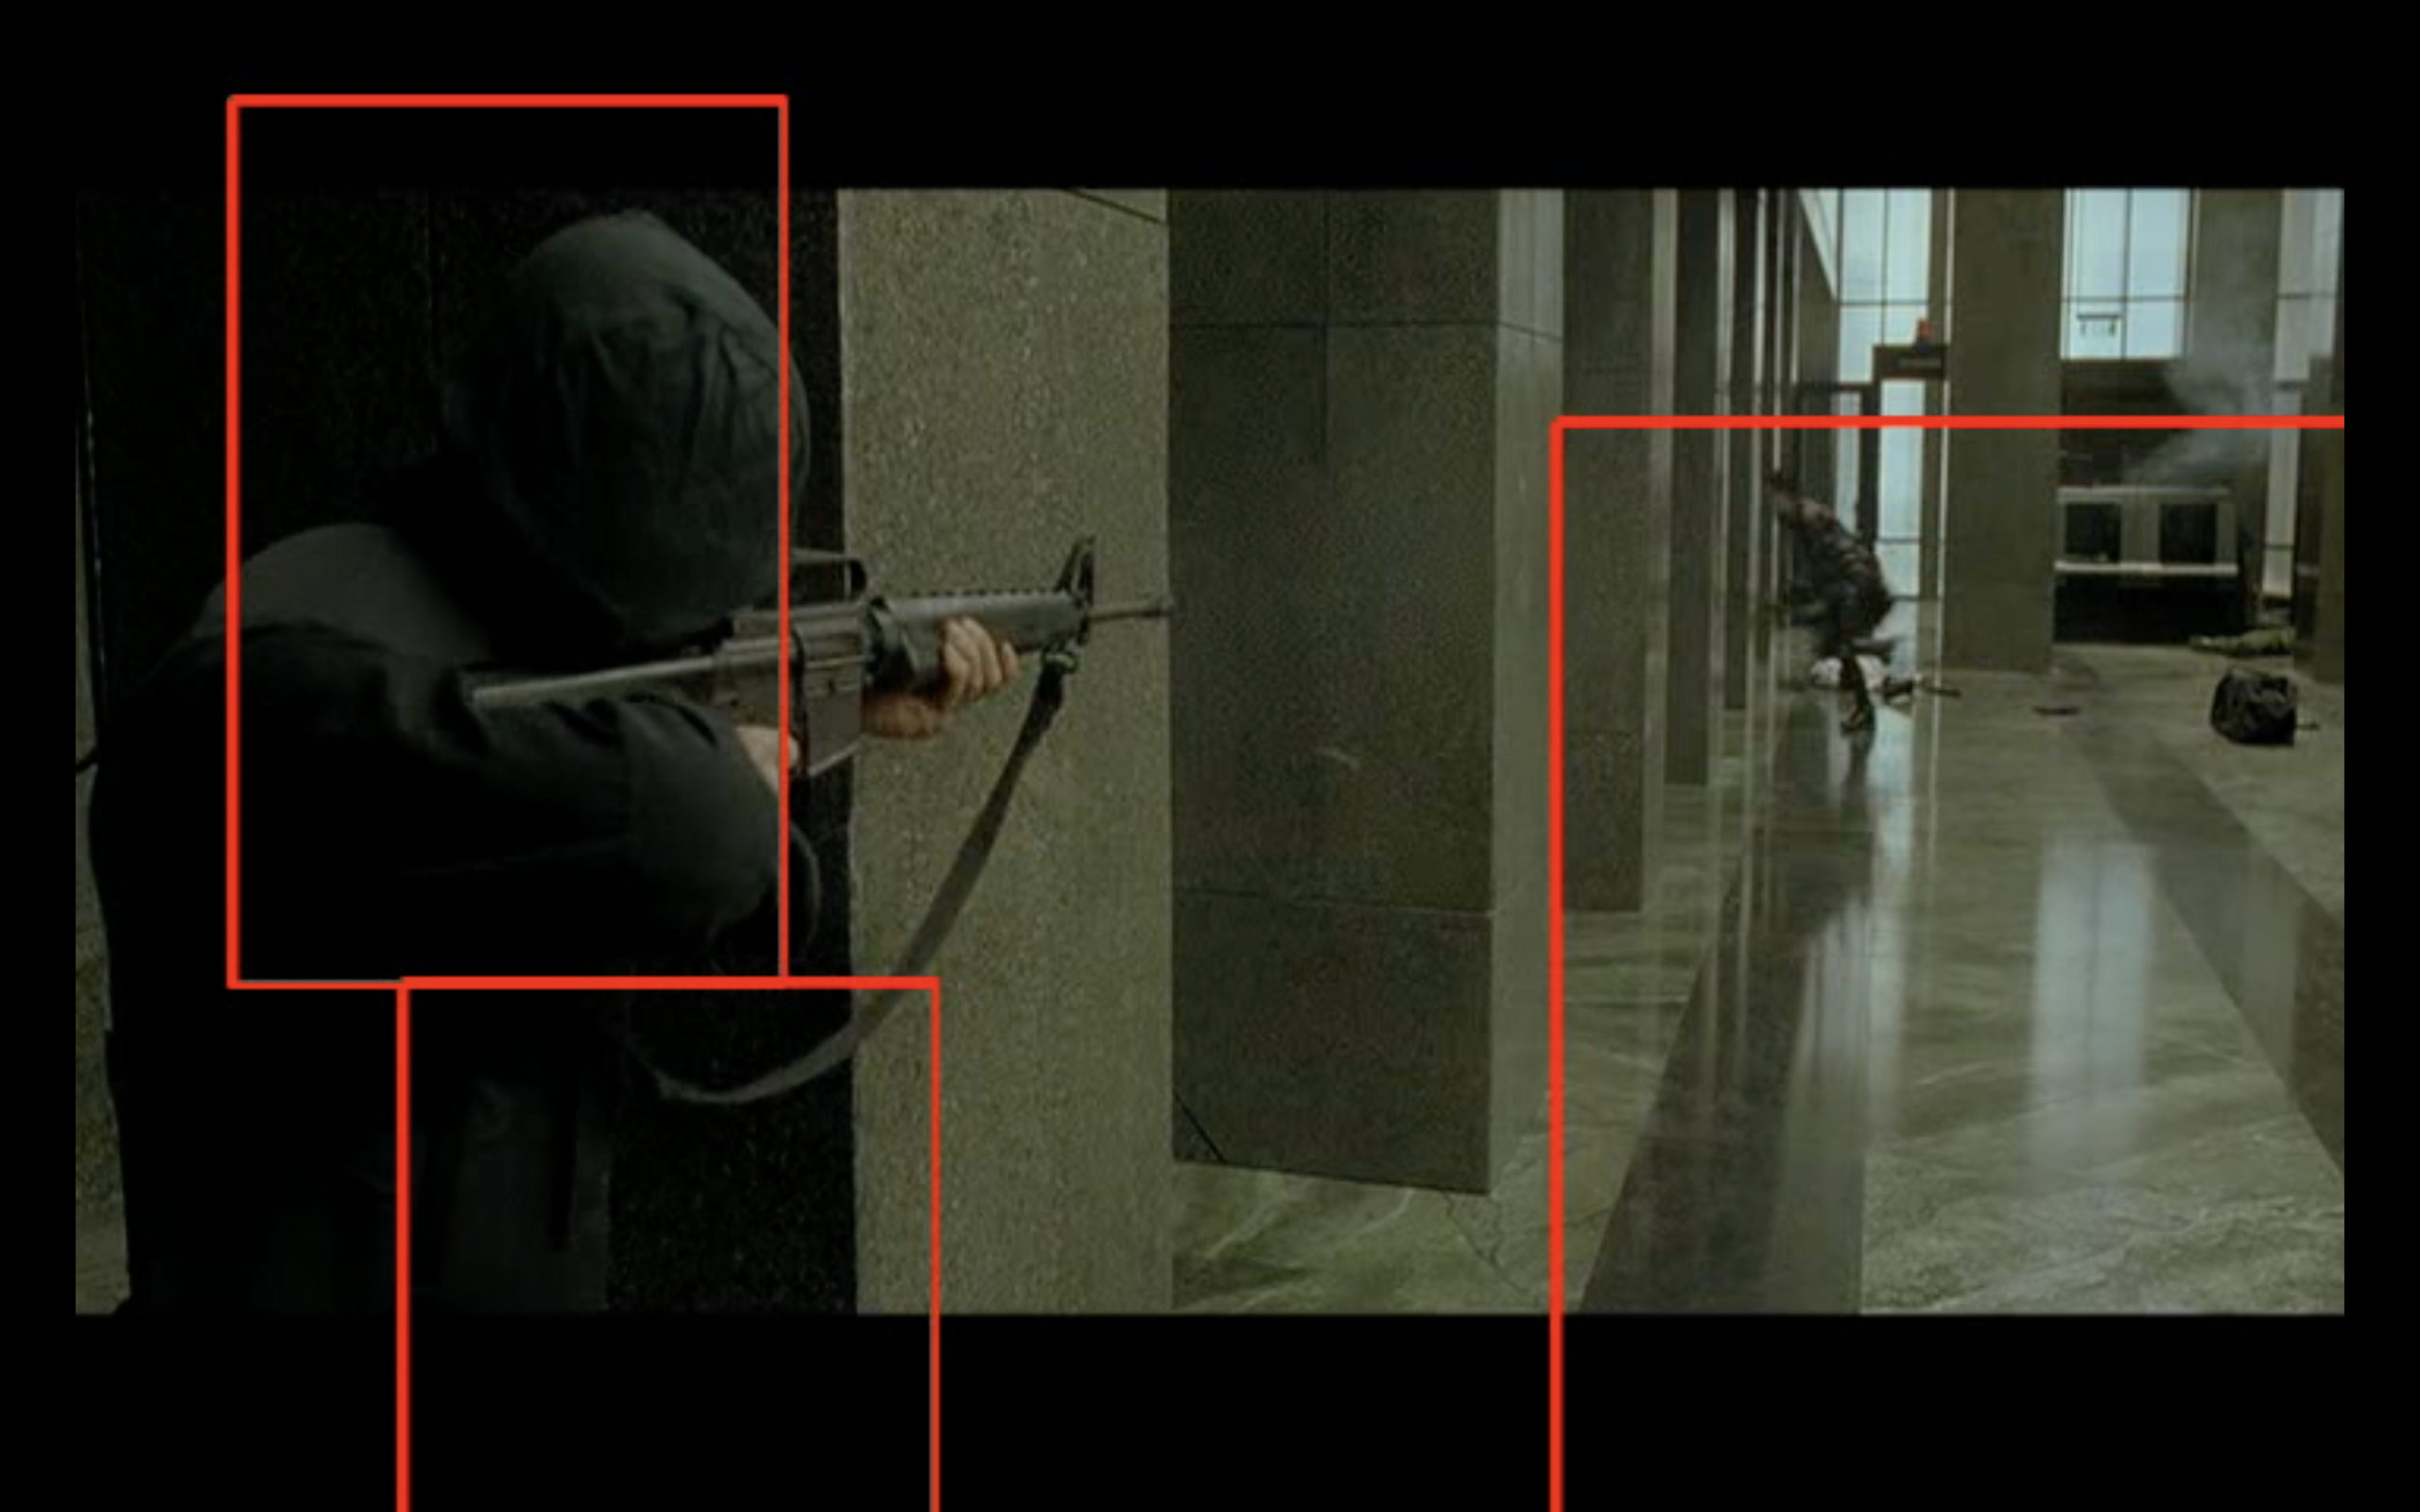
\includegraphics[width=0.4\columnwidth]{pedestrian1.png}
        \caption{\label{fig4} Pedestrian Open-CV HOG detection
        }
\end{figure}

\begin{figure}[ht] 
        \centering 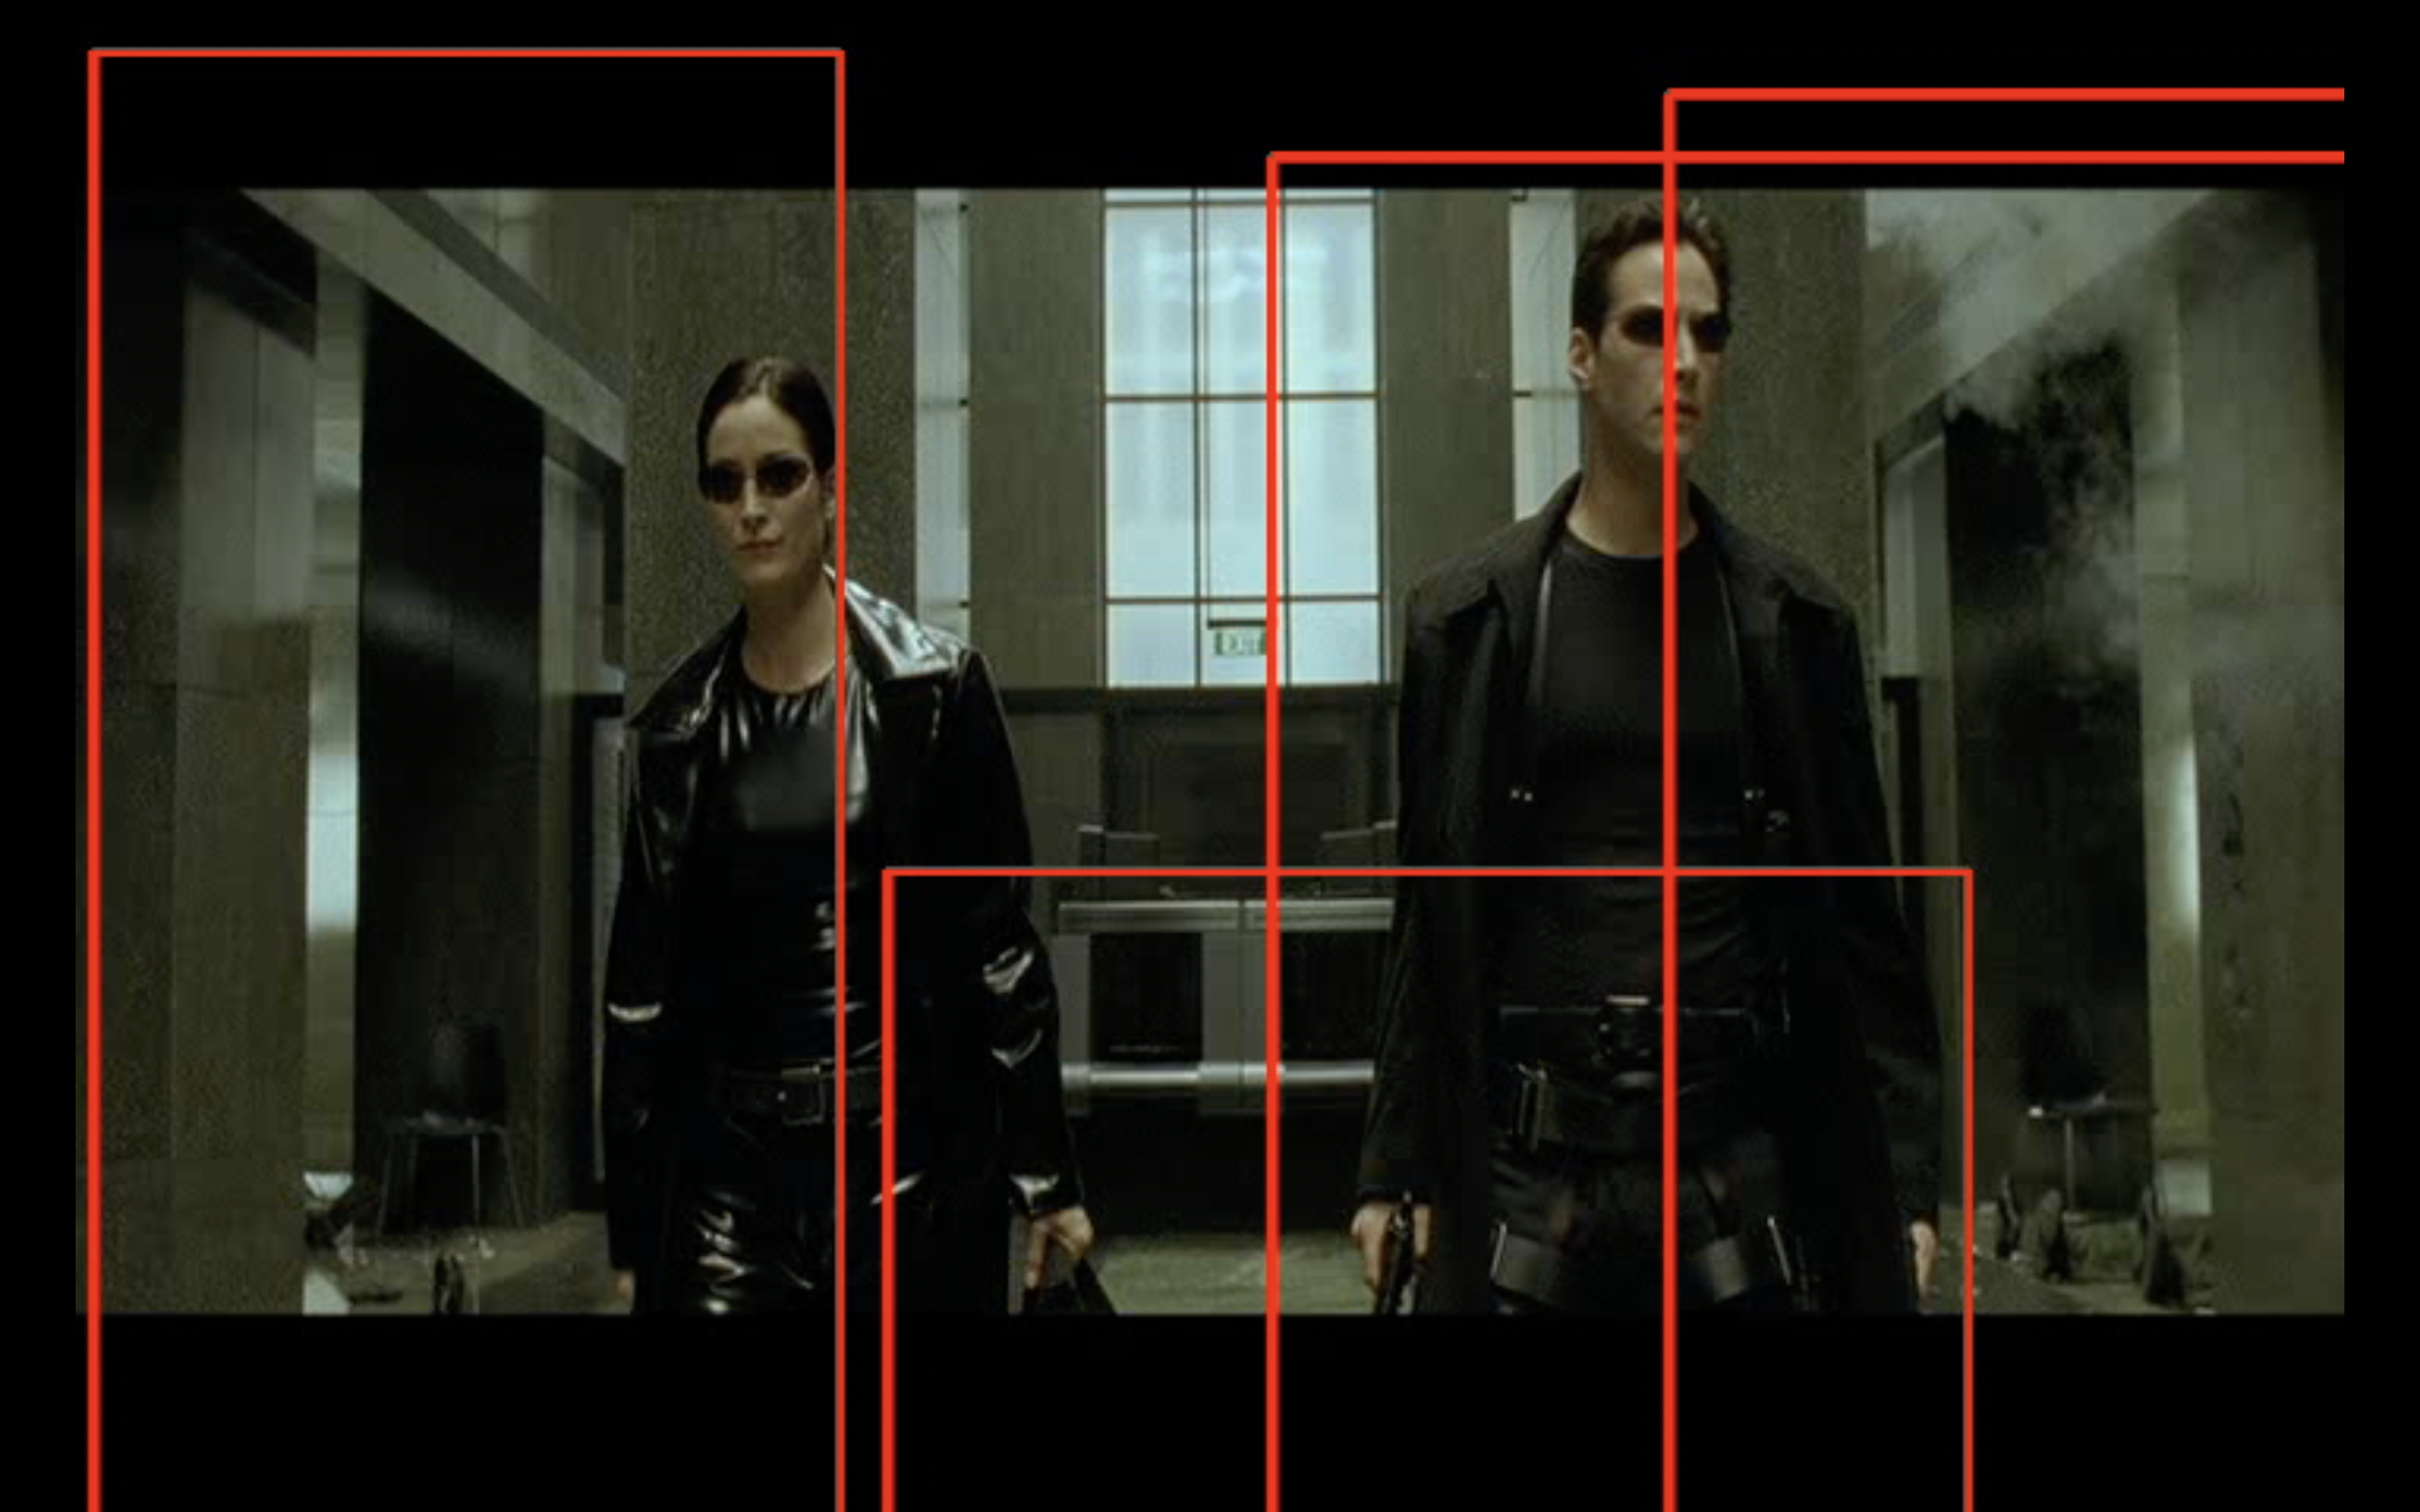
\includegraphics[width=0.4\columnwidth]{pedestrian2.png}
        \caption{\label{fig5} Pedestrian Open-CV HOG detection
        }
\end{figure}

Face detection varied for different bitrates, with the miss rate decreasing with increasing bitrate. There were exactly 700 faces detected in the 2000 frames video. On the 500Kb/s video the miss rate was 0.81, on the 1000KB/s video the miss rate was 0.93, and on the 2000 KB/s video the miss rate was 0.97. The histograms for a lower bitrate videos changed, resulting in less recognized pattern of face(see Figures \ref{fig6}).

\begin{figure}[ht] 
        \centering \includegraphics[width=0.8\columnwidth]{HOG500K200K.png}
        \caption{\label{fig6} HOG for face detection 500Kb/s vs 2000Kb/s
        }
\end{figure}

For the pedestrian detection using Detectron2, the miss rate for 2000 Kb/s was 0.91, for 1000 Kb/s - 0.83, for 500 Kb/s - 0.74. The relatively highest number of false positives was observed in the scene where the image degradation was the highest (see Figures \ref{fig7}).

\begin{figure}[ht] 
        \centering \includegraphics[width=0.8\columnwidth]{detectron.png}
        \caption{\label{fig7} Detectron2 person detection 500Kb/s vs 2000 Kb/s
        }
\end{figure}

The results for Face and Pedestrian detection performance are on Table~\ref{table1}.

\begin{table}[ht]
\begin{center}
\caption{Miss rate for face and pedestrian recognition in different bitrate videos}
\label{table1} 
\begin{tabular}{cccc} %change to cc for 2 columns
\hline
\multicolumn{1}{c}{Detection Model} & 
\multicolumn{1}{c}{Bitrate 500Kb/s} & 
\multicolumn{1}{c}{Bitrate 1000Kb/s} & 
\multicolumn{1}{c}{Bitrate 2000Kb/s} \\
\hline
HOG (Face) & 0.81 & 0.93 & 0.97 \\
Detectron2 & 0.74 & 0.83 & 0.91 \\
\hline
\end{tabular}
\end{center}
\end{table}




The main difference between detecting objects on videos and photos is that the movements of the objects can be used to gain extra information for their detection and classification. The very first task in video analysis is the estimation of motion or optical flow. Optical flow refers to the vector field of the apparent movement of pixels between frames. At the same time, Motion Estimation does the same task and is the first module of a video encoder. Since consecutive video frames include large amounts of same data, and differ only by moving objects, a next frame can be reconstructed from the previous one. The motion vectors used for the reconstruction can be also used for locating the object in the next frame, if an object was recognized successfully in the original one. 

However, preparing datasets for Optical Flow based object detectors classifiers is a hard task, and not many of such datasets exist. One practical dataset currently in use is the KITTY dataset for self-driving cars. The approach of using Optical Flow based detectors provides better accuracy than our solution, but requires more time for creating dataset.

The other disadvantage of our solution is running time, which can be decreased slightly by using Visual Object Tracking (VOT).For example, every 5 frames a detector is applied, and in the intermediate frames, the face is tracked as a small fragment through a pattern matching method. This approach is used in GOTURN (Generic Object Tracking Using Regression Networks).

\section{Conclusion}




\cite{article1}


\bibliographystyle{plainnat}
\bibliography{references.bib}

\appendix


\end{document}
